\chapter{Evaluation}

Um es zu überprüfen, ob die Ziele dieses Projektes erreicht werden, wird eine Studie durchgeführt. In diesem Kapitel geht es um den Entwurf der Studie und die Analyse über der gesammelten Daten.

\section{Entwurf der Studie}

Die Hauptziele der Studie sind, den Lerneffekt der VR Übung und die Benutzererfahrung der WebVR Applikation zu beurteilen. Die Studie wird um die Ziele herum entworfen.

\subsection{Entwurf des Tests und des Fragebogens}

Das Projekt wird hinsichtlich zweier Aspekte getestet: der Lerneffekt der VR Übung und die Benutzererfahrung der VR Applikation. Deswegen werden die Teile der Studie für jeden Aspekt getrennt entworfen.

\subsubsection{Lerneffekt durch die VR Übung}

Da die VR Übung in dem Learning Management System Moodle integriert wird, kann der Lerneffekt durch die Test Aktivität überprüft werden. Fünf Aufgaben werden in der Test Aktivität eingefügt, damit kann von der Reihenfolge der Infusinosvorbereitung bis kleine Forderung eines Abschnitts überprüft werden.

\begin{enumerate}
    \item \textbf{Reihenfolge ordnen}
    
    Die acht Abschnitte der Infusionsvorbereitung werden ungeordnet dargestellt. Sie sollen nach der richtigen Reihenfolge geordnet werden. Durch diese Aufgabe wird geprüft, ob sich der Lernende den Ablauf einer Infusionsvorbereitung eingeprägt hat. (Abbildung ~\ref{fig:Aufgabe1})
    
\begin{figure}[ht]
\vspace*{1em}
\centering
\caption{Aufgabe: Reihenfolge}
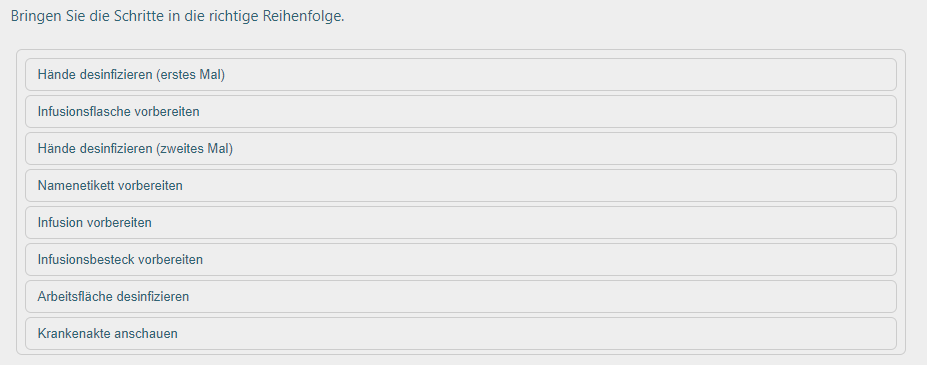
\includegraphics[width=\textwidth]{images/Aufgabe1.png}
\label{fig:Aufgabe1} 
\end{figure}
    
    
    \item \textbf{5R auswählen}
    
    5R sind die wichtigen Informationen auf der Krankenakte, die während der Vorbereitung zuerst geprüft werden sollen. Fünf richtige Optionen sollen aus acht Optionen ausgewählt werden. Durch diese Aufgabe wird geprüft, ob der Lernende gelernt hat, was die wichtigen Informationen für die Infusionsvorbereitung sind. (Abbildung ~\ref{fig:Aufgabe2})
    
\begin{figure}[ht]
\vspace*{1em}
\centering
\caption{Aufgabe: 5R-Regel}
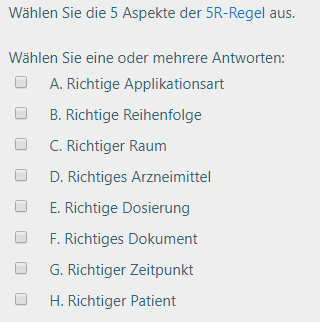
\includegraphics[width= 0.5\textwidth]{images/Aufgabe2.png}
\label{fig:Aufgabe2} 
\end{figure}
    
    \item \textbf{Status der Rollenkleme}
    
    Während der Infusionsvorbereitung ist es wichtig, die Rollenklemme zu den entsprechenden Zeitpunkten zu öffnen und zu schließen. Durch die Aufgabe wird überprüft, ob sich der Lernende die richtigen Zeitpunkte gemerkt hat. (Abbildung ~\ref{fig:Aufgabe3})
    
\begin{figure}[ht]
\vspace*{1em}
\centering
\caption{Aufgabe: Rollenklemme}

\includegraphics[width= \textwidth]{images/Aufgabe3.png}
\label{fig:Aufgabe3} 
\end{figure}
    
    \item \textbf{Handschuhe tragen}
    Hygiene und Sicherheit sind wichtige Themen. Durch Handschuhe werden nicht nur die Hände geschützt, sondern auch die Handlung hygienisch durchgeführt. Die Übung besteht aus acht Abschnitten, wobei eine davon ausgewählt werden soll, bei der  Handschuhe getragen werden. Durch diese Aufgabe werden das Sicherheitsbewusstsein und das Hygienebewusstsein der Lernenden überprüft. (Abbildung ~\ref{fig:Aufgabe4})
    
\begin{figure}[ht]
\vspace*{1em}
\centering
\caption{Aufgabe: Handschuhe}
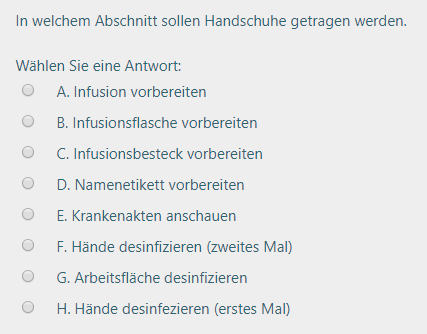
\includegraphics[width= 0.5\textwidth]{images/Aufgabe4.png}
\label{fig:Aufgabe4} 
\end{figure}
    
    \item \textbf{Infusionsflasche prüfen}
    
    Um die Nutzbarkeit der Infusionsflasche zu bestimmen, soll die Infusionsflasche vor der Nutzung geprüft werden, nämlich die Kappe, die Flüssigkeit und das Etikett. Vier Optionen werden aufgelistet, und die drei richtigen Optionen sollen ausgewählt werden. Durch diese Aufgabe wird es überprüft, ob der Lernende das Bewusstsein hat, die Benutzbarkeit der Materialien zu prüfen. (Abbildung ~\ref{fig:Aufgabe5})
    
\begin{figure}[ht]
\vspace*{1em}
\centering
\caption{Aufgabe: Handschuhe}
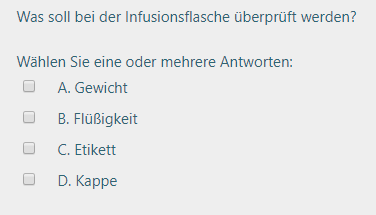
\includegraphics[width= 0.5\textwidth]{images/Aufgabe5.png}
\label{fig:Aufgabe5} 
\end{figure}
    
\end{enumerate}

\subsubsection{Benutzererfahrung der VR Applikation}

Die Benutzererfahrung ist ziemlich subjektiv, deswegen wird ein Fragebogen erstellt, um das Feedback der Benutzer zu sammeln.

Um die Benutzererfahrung umfassend zu berichten, wird der Fragebogen nach den sechs Kategorien \citep{28} entworfen. Da die Benutzererfahrung zusammengefasst ist, ist es schwierig, nach jeder einzigen Kategorie Fragen zu stellen. Deswegen können die Fragen auch mehrere Kategorien betreffen.

Jede Frage besteht aus zwei Teilen. Einer davon ist eine Pflicht-Frage im Form von Ratingskalen. Der andere ist eine entsprechende optionale Frage im Form einer Meinungsfrage.

\begin{enumerate}
    \item Ich habe das Gefühl, wirklich eine Infusion vorzubereiten.
    
    Wenn nein, was ist die Ursache (z.B. Mangel an Geräuschen)?
    
    (Extensiveness, Matching, Surroundness, Vividness, Interactability)
    
    \item Während der Übung weiß ich, was und wie ich es tun soll.
    
    Wenn nein, was ist unklar?
    
    (Interactability, Plot)
    
    \item Ich kann das Zielobjekt mühelos finden.
    
    Wenn nein, was ist nicht einfach zu finden?
    
    (Matching, Surroundness, Vividness)
    
%    \item Ich bin immer sicher, dass jede Aktion von mir auf den Objekten durchgeführt wird. Wenn das Objekt nicht reagiert, kann mit dem Objekt auch nicht interagiert werden.
%    
%    Wenn nein, was funktioniert nicht?
%    
%    (Interactability, Plot)
    
    \item  Das Feedback der Objekte nach der Interaktion habe ich erwartet. 
    
    Wenn nein, was ist unerwartet?
    
    (Matching, Interactability)
    
%    \item Ich kann die wichtige Informationen (z.B. 5R, Etiketten) deutlich sehen.
%    
%    Wenn nein, was ist undeutlich?
%    
%    (Surroundness, Vividness)
    
\end{enumerate}

Whiteboard wird als Hilfsmittel entworfen. Um den Effekt des Whiteboards zu untersuchen, werden die Fragen über die Nutzung des Whiteboards in den Formen Entscheidungsfragen und Ratingskalen gestellt.

\begin{enumerate}
    \item Ich habe die Hinweise auf dem Whiteboard benutzt.
    
    Wenn ja, sind die Hinweise hilfreich?
\end{enumerate}

Für das ganze Projekt werden die Fragen über der Integration zwischen LMS und die WebVR Applikation in den Formen Ratingskalen und Meinungsfrage und die Frage über dem Lerneffekt im Form Ratingskalen gestellt.

\begin{enumerate}
    \item Ich glaube, dass die VR Übung gut in den Unterricht integriert ist.
    
    Wenn nein, was gefällt Ihnen nicht?
%    
%    \item Wie gut ist der Lerneffekt im Vergleich mit der realen Praxis? 
\end{enumerate}

Am Ende des Fragebogens werden zwei allgemeine Meinungsfragen gestellt, um die Gedanken der Versuchspersonen zu sammeln.

\begin{enumerate}
    \item Was gefällt Ihnen während der Übung?
    
    \item Was gefällt Ihnen während der Übung nicht?
\end{enumerate}

\subsection{Entscheidung der Geräten}

Da WebVR eine cross-plattform ist, wird die Studie mit unterschiedlichen Geräten gemacht. Allerdings ist es wegen der Begrenzung der Zeit und des Mangels an Versuchspersonen nicht möglich, mit allen verfügbaren Geräten die Studie zu machen, deswegen werden drei Geräte zur Studie gewählt.

\begin{itemize}
    \item \textbf{PC}: beste Erreichbarkeit
    \item \textbf{Smartphone}: beste Mobilität
    \item \textbf{HTC Vive}: bestes VR Erlebnis
\end{itemize}

\subsection{Entwurf des Ablaufs}

Insgesamt 15 Versuchspersonen nehmen an der Studie teil. Sie haben kein Vorwissen über Infusionsvorbereitung, damit kann der Lerneffekt des Unterrichts und der VR Übung berichtet werden.

Jedes Gerät wird von fünf Versuchspersonen benutzt. Jede Versuchsperson soll die Untersuchung allein machen.

Die Versuchsperson wird gefordert, zuerst mit den drei Materialien (Text, Video und Diagramm) zu lernen, und den Test zu machen. Das Ergebnis des Tests wird nicht der Versuchsperson mitgeteilt, sondern als Controllergruppe gespeichert.

Danach soll die Versuchsperson die VR Übung machen und den Test noch einmal machen. Die Zwei Ergebnisse werden miteinander verglichen, um den Effekt der Übung zu finden.

Am Ende der Studie soll die Versuchsperson einen Fragebogen ausfüllen, um die Benutzererfahrung der WebVR Applikation zu beurteilen.

\section{Daten der Studie}

Insgesamt vier Männer und elf Frauen haben an der Studie teilgenommen. Zehn Versuchspersonen studieren an der Universität Bielefeld oder Fachhochschule Bielefeld. Fünf Versuchspersonen haben das Studium an der Universität Bielefeld abgeschlossen. Das durchschnittliche Alter ist 27.

Die Daten werden durch den Test und den Fragebogen gesammelt, die den Lerneffekt und die Benutzererfahrung der VR Übung widerspiegeln. Hier werden die auffälligen Daten gelistet.

\subsection{Lerneffekt}

Nach dem Lernen mit dem Unterricht können die Versuchspersonen mindesten 84 Punkte von 100 Punkte erwerben. Besonders wenn mit PC oder HTC Vive gelernt wurde, können über 90 Punkte erreicht werden. (Abbildung ~\ref{fig:testErgebnisse})

Die Testergebnisse nach der VR Übung für alle Geräte sind deutlich besser als vor der VR Übung. Die Verbesserungen mit PC (44.0\%) und HTC Vive (43.3\%) sind fast gleich und viel gravierender als mit dem Smartphone (12.9\%).

\begin{figure}[ht]
\vspace*{2.3em}
\centering
\caption{Vergleich des Lerneffektes}
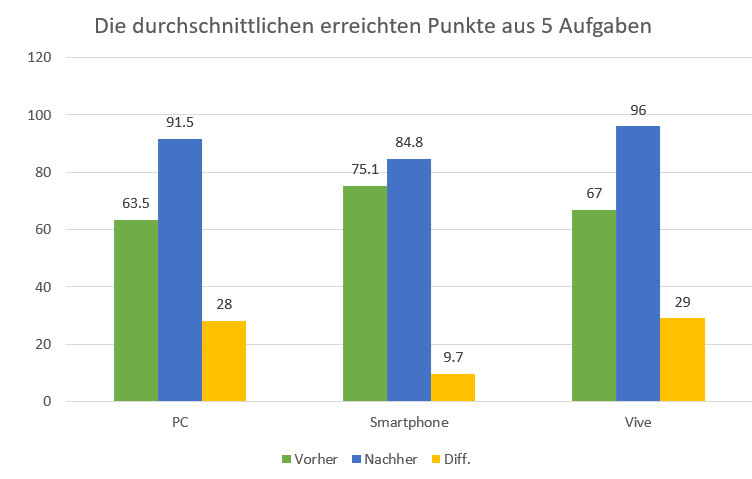
\includegraphics[width= \textwidth]{images/testErgebnisse.png}
\label{fig:testErgebnisse}
\vspace*{1em}
\end{figure}

\subsection{Benutzererfahrung}

Die Vive Benutzer haben fast ein identisches Gefühl von Immersion, alle haben sich auf der Skala für den Wert 4 oder 5 entschieden. Obwohl das immersive Gefühl für die PC Benutzer auch stark ist, sind die Meinungen nicht einstimmig. Das immersive Gefühl für die Smartphone Benutzer ist nicht so stark wie die Benutzer mit den anderen zwei Geräten. (Abbildung ~\ref{fig:gefuehlWirklich})

\begin{figure}[ht]
\vspace*{1em}
\centering
\caption{Ergebnisse für Immersion}
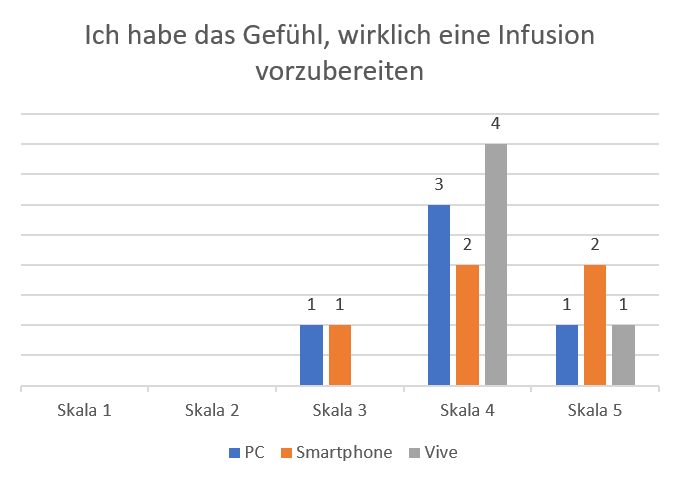
\includegraphics[width= \textwidth]{images/gefuehlWirklich.png}
\label{fig:gefuehlWirklich} 
\end{figure}

Alle Versuchspersonen haben positives Feedback gegeben, wenn gefragt wird, ob sie wissen, was und wie es zu tun ist. (Abbildung ~\ref{fig:wasWie})

\begin{figure}[ht]
\vspace*{1em}
\centering
\caption{Was und Wie zu tun}
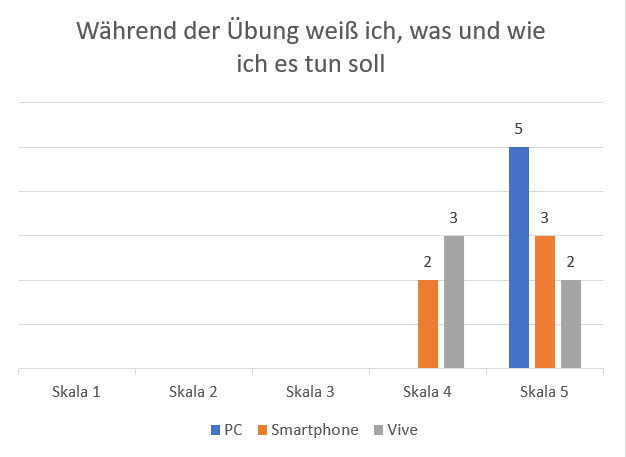
\includegraphics[width= \textwidth]{images/wasWie.png}
\label{fig:wasWie} 
\end{figure}

Die PC und Vive Benutzer können die Zielobjekte ziemlich mühelos finden. Allerdings ist es nicht einfach für die Smartphone Benutzer, zwei von fünf Smartphone Benutzern haben negatives Feedback gegeben. (Abbildung ~\ref{fig:muehelosFinden})

\begin{figure}[ht]
\vspace*{1em}
\centering
\caption{Zielobjekte finden}
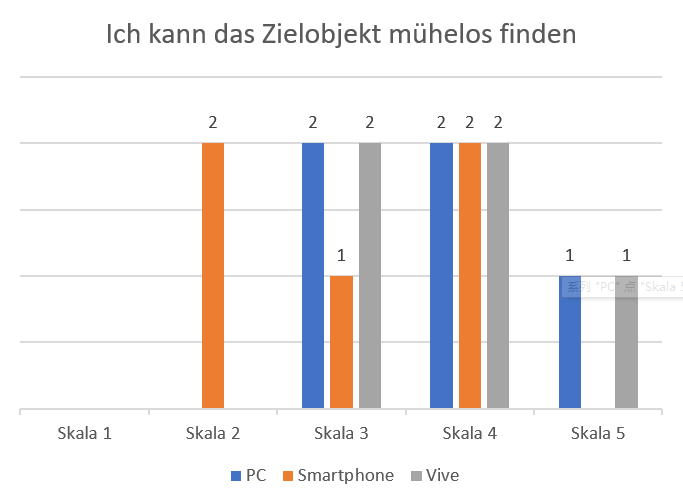
\includegraphics[width= \textwidth]{images/mueelosFinden.png}
\label{fig:muehelosFinden} 
\end{figure}

Alle Vive Benutzer haben die beste Bewertung für das Feedback der Objekte gegeben. Obwohl die meisten Benutzer von PC und Smartphone auch die beste Beurteilung gegeben haben, denken drei Benutzer, dass die Reaktionen der Objekte nicht ganz ihren Erwartungen entsprechen. (Abbildung ~\ref{fig:feedbacksDerObjekte})

\begin{figure}[ht]
\vspace*{1em}
\centering
\caption{Feedback der Objekte}
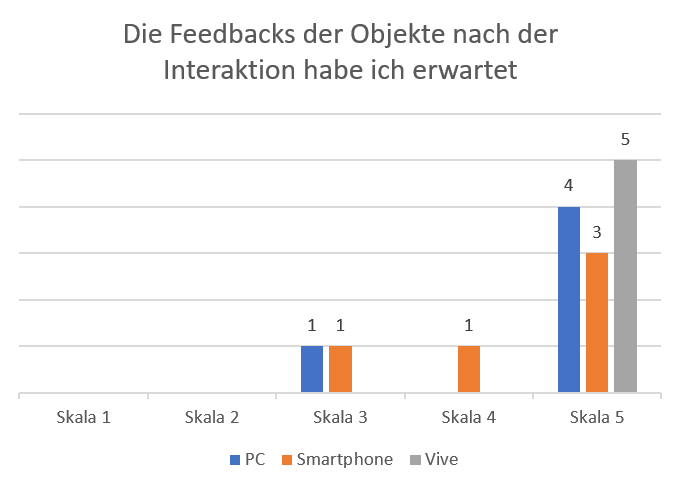
\includegraphics[width= \textwidth]{images/feedbacksDerObjekte.png}
\label{fig:feedbacksDerObjekte} 
\end{figure}

\section{Diskussion}

Durch die Analyse der gesammelten Daten, werden die Erfolge und die Probleme des Projektes gefunden.

\subsection{Erfolge}

\begin{itemize}
    \item \textbf{Lerneffekt der VR Übung}
    
    Der Fortschritt nach der VR Übung ist deutlich, 10 bis 29 Punkte werden mehr erworben. Es passiert während der Studie zwei Mal, dass die Versuchsperson bei dem erstmaligen Test schon alle Fragen richtig beantwortet hat. Allerdings habe sie die Erfahrung, dass sie nicht 100\% sicher für die Antworten bei dem erstmaligen Test ist. Nach der VR Übung kam die Überzeugen, dass sie alle Punkte kriegen könnten.
    
    \item \textbf{Hinweise auf dem Whiteboard}
    
    Alle Versuchspersonen haben die Hinweise benutzt und glauben, dass die Hinweise sehr hilfreich sind.
    
    \item \textbf{Integration der VR Übung in den Unterricht}
    
    Alle Versuchspersonen sind der Meinung, dass die VR Übung sehr gut in den Unterricht integriert wird. Inhaltlich wiederholt die VR Übung die Kenntnisse. Äußerlich gilt die VR Übung als eine Aktivität des Unterrichts.
    
    \item \textbf{Geräusche Feedbacks}
    
    Es kann passieren, dass es keine Reaktion des Zielobjektes nach der Interaktion gibt, deswegen gelten die Geräusche als zuverlässiges Feedback für jede Interaktion.
    
\end{itemize}

\subsection{Probleme}
\begin{itemize}
    \item \textbf{Objekte schwer zu finden (Smartphone > PC > Vive)}
    
    Das Problem erscheint auf allen drei Geräten. Das Problem auf Smartphone und PC ist dabei gravirender als auf HTC Vive. Es gibt zwei Gründe für die Schwierigkeit, die Objekte zu finden.
    
    Der erste Grund ist, dass die Umgebung und die Objekte für die Versuchspersonen, die keine Pflege-Studenten sind, fremd sind. Es passiert mehrere Male, dass die Versuchspersonen nicht wissen, wo die Krankenakte und die Einmalhandschuhe abgelegt werden, weil die Krankenakte geschlossen ist und der Spender für Einmalhandschuhe nicht bekannt ist.
    
    Der zweite Grund ist, dass die Ansicht der Smartphones klein ist. Die Hängeschränke sind sogar nicht in der Sicht des Smartphones nach der Initialisierung.
    
    Um das Problem zu lösen, sollen die Umgebung und die Objekte in den Unterricht als Vorwissen vorgestellt werden, oder soll eine Leitung über der Umgebung und den Objekten in der VR Umgebung vor dem Start der Übung geboten werden.
  
    \item \textbf{Fehlen des aktiven Hinweises}
    
    In der VR Umgebung werden die Hinweise durch das Whiteboard dargestellt. Allerdings ist es ein passives Angebot. Das heißt, dass die Hinweise ignoriert werden, wenn der Benutzer nicht zum Whiteboard schaut. Deswegen passiert es, dass sich die Versuchsperson lange Zeit auf ein falsches Objektes konzentriert, weil er nicht rechtzeitig an das Whiteboard schaut.
    
    Um das Problem zu lösen, soll ein aktiver Hinweis eingesetzt werden, d.h. direkt vor den Augen in den richtigen Zeiträumen darzustellen. Der Hinweis kann ein Vorschlag sein, das Whiteboard anzuschauen.
    
    \item \textbf{Die Entfernung der Einmalhandschuhe nicht deutlich}
    
    Nach der Desinfektion der Arbeitsfläche werden die Merkmale der Einmalhandschuhe (Einmalhandschuhe Modell vor den Augen in PC und Smartphone und blauer Farbe auf die Hände in Vive) entfernt. Aber die Entfernung ist nicht deutlich, weil es keine Animation dafür gibt. Sodass manche Versuchspersonen nicht merken, wann die Handschuhe entfernt werden.
    
    Mit einer Animation für die Entfernung kann das Problem behoben werden.
    
    \item \textbf{Fehlen des Feedback nach der Prüfung für Infusionsflasche und Infusionsbesteck mit PC und Smartphone}
    
    Wenn PC und Smartphone benutzt werden, gelten die Bewegungen der Infusionsflasche und der Infusionsbesteck als die Feedbacks der Prüfung anstelle des Haken auf den geprüften Positionen. Allerdings ist ein solches Feedback nicht deutlich, sodass die Schwerpunkte der Überprüfung nicht gemerkt werden.
    
    Um das Problem zu lösen, sollen die Haken nach der entsprechenden Prüfung dargestellt werden.
\end{itemize}












